% !TEX root = main.tex

\section{Part 2: Identification of wave spectrum model}

\subsection{2a)}

% Si noe om hva oppgaven er (finne \omega_0 og \lambda)

To estimate the Power Spectral Density, we use Welch's estimate, which is implemented in Matlab as seen in \cref{lst:p2}. The result is included in \cref{fig:PSD}.

\lstinputlisting[language=Matlab, basicstyle=\small, caption={The Matlab code used in part 2}, label={lst:p2},float]{listings/estimate_psd.m}

\subsection{2b)}
To find the values of $\omega_0$ and $\lambda$ we can compare the estimated PSD of the waves with an analytical, found by using the model of the waves. In order to do this we first need to find the transfer function from $w_w$ to $\psi_w$. This can be done by taking the laplace transform of \cref{eq:xi_w} and \cref{eq:psi_w} yielding

\begin{equation}
    G(s) = \frac{\psi_w}{w_w}(s) = K_w\frac{s}{s^2+2\lambda\omega_0s+\omega_0^2} \label{eq:G(s)}
\end{equation}

To find the power spectral density function we use that $S_y(\omega) = |H(j\omega)|^2S_u(\omega)$. This means

\begin{equation}
    P_{\psi_w}(\omega) = |G(j\omega)|^2 = K_w^2\frac{\omega^2}{\omega^4+2\omega_0^2(2\lambda^2-1)\omega^2+\omega_0^4} \label{eq:PSD}
\end{equation}


\subsection{2c)}

$\omega_0$ was estimated as the maximum frequency in the PSD estimate, as shown in \cref{lst:p2}. This frequency is $0.7823\si{\Hz}$.

\subsection{2d)}

$\lambda$ was estimated using the Matlab function \texttt{lsqcurvefit}, which iterates toward the $\lambda$ that yields a curve closest to the PSD estimate. The resulting $\lambda$ is $0.0827$.

The PSD of the model, using these parameters, together with the PSD estimate from the data, is plotted in \cref{fig:PSD}.

\begin{figure}
	\centering
	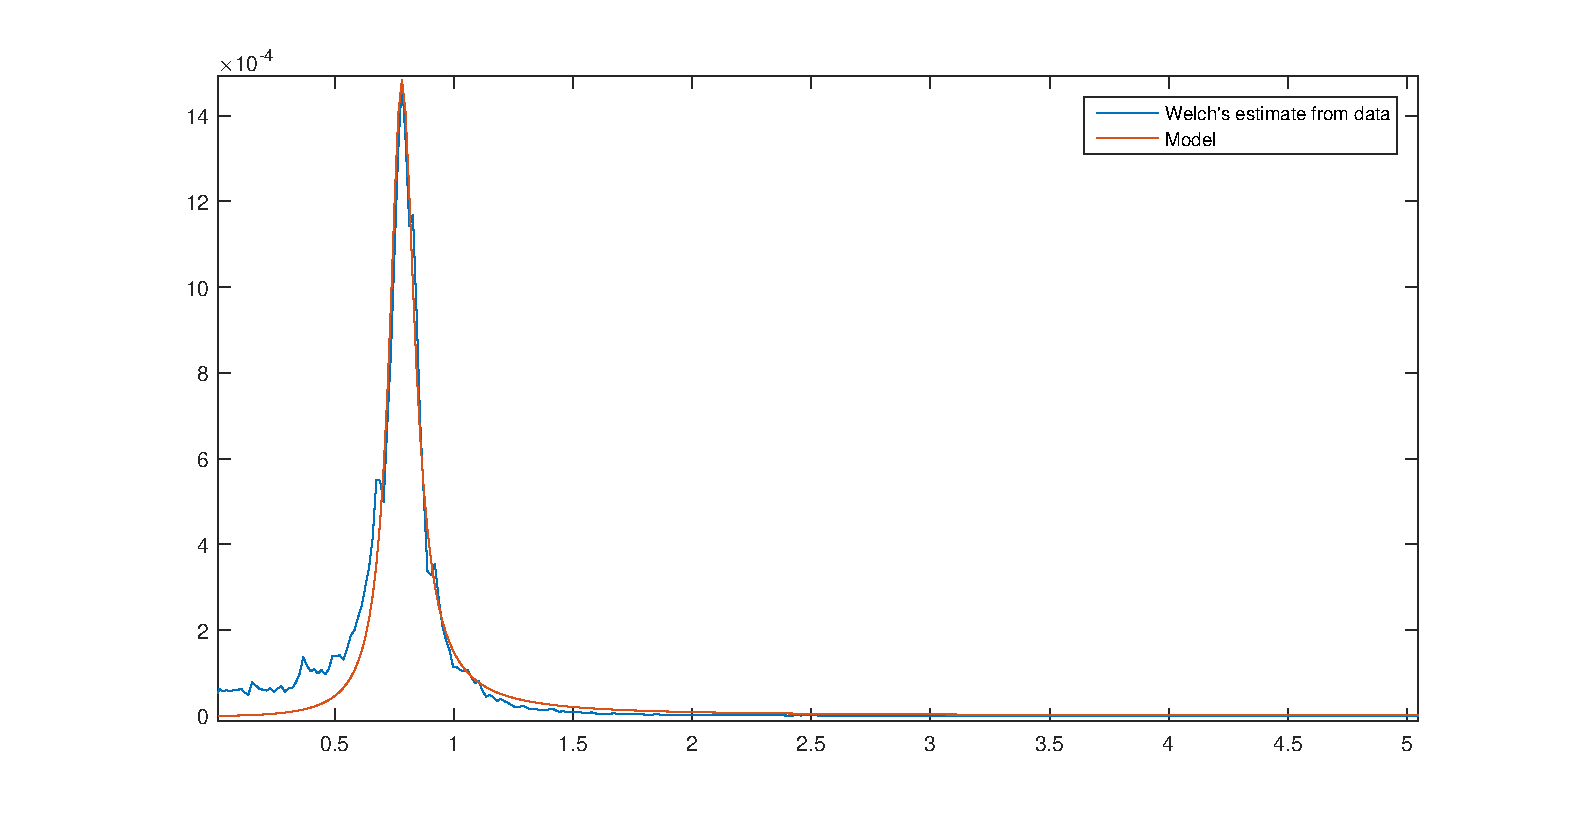
\includegraphics[width=\textwidth]{images/oppg2/PSD}
	\caption{Estimated PSD from data and PSD of model.}
	\label{fig:PSD}
\end{figure}
